\documentclass[12pt,a4paper]{article}

% ------------------------------------------------------------
% Pacotes
% ------------------------------------------------------------
\usepackage[T1]{fontenc}
\usepackage[utf8]{inputenc}
\usepackage{lmodern}
\IfFileExists{brazil.ldf}{\usepackage[brazil]{babel}}{}
\usepackage[a4paper,top=3cm,left=3cm,right=2cm,bottom=2cm,headheight=15pt]{geometry}
\usepackage{amsmath,amssymb,amsthm}
\usepackage{booktabs}
\usepackage{tikz}
\usepackage{caption}
\usepackage{fancyhdr}
\usepackage{setspace}
\usepackage{indentfirst}
\usepackage[hidelinks]{hyperref}
\usepackage{graphicx}


\renewcommand{\contentsname}{Sumário}
\renewcommand{\refname}{Referências}
\renewcommand{\figurename}{Figura}
\renewcommand{\tablename}{Tabela}
\renewcommand{\abstractname}{Resumo}
\renewcommand{\proofname}{Demonstração}

\onehalfspacing
\setlength{\parindent}{1.25cm}

\pagestyle{fancy}
\fancyhf{}
\fancyhead[R]{\small Paradoxo da Amizade}
\fancyfoot[C]{\thepage}

\theoremstyle{plain}
\newtheorem{teorema}{Teorema}
\newtheorem{lema}{Lema}
\theoremstyle{definition}
\newtheorem{definicao}{Definição}
\theoremstyle{remark}
\newtheorem{observacao}{Observação}

\captionsetup{font=small,labelsep=endash}

% Notação
\newcommand{\dm}{\bar d}          % média por pessoa
\newcommand{\dA}{\bar d_{A}}      % média na lista de amigos
\newcommand{\dI}{\bar d_{I}}      % média por indicação

% Estilo dos desenhos de grafos
\tikzset{
  v/.style={circle,draw=blue!50!black,fill=blue!10,minimum size=6mm,inner sep=0pt,font=\small},
  e/.style={draw=black!70,thick}
}

\begin{document}

% ------------------------------------------------------------
% Capa
% ------------------------------------------------------------
\begin{titlepage}
\centering
\onehalfspacing
{\large FUNDAÇÃO GETULIO VARGAS\\
ESCOLA DE MATEMÁTICA APLICADA -- FGV EMAp\par}
\vspace{3cm}
{\large Ana Alice Silva\\ Henrique Lara\\ Mayara Ap.\ P.\ Bomback\par}
\vspace{3.5cm}
{\Large\bfseries O PARADOXO DA AMIZADE:\\[0.3em]
POR QUE SEUS AMIGOS PARECEM TER\\ MAIS AMIGOS DO QUE VOCÊ\par}
\vspace{3cm}
\begin{minipage}{0.7\textwidth}
\centering\small\singlespacing
Trabalho apresentado à disciplina de Matemática Discreta da Escola de
Matemática Aplicada da Fundação Getulio Vargas.\\[0.6em]
Professora: Maria Soledad Aronna\\
Ciência de Dados, 2º período
\end{minipage}
\vfill
{\large Rio de Janeiro\\ 2026\par}
\end{titlepage}

% ------------------------------------------------------------
% Resumo
% ------------------------------------------------------------
\pagenumbering{roman}

\section*{Resumo}

Este trabalho investiga o Paradoxo da Amizade por meio da
teoria dos grafos, demonstrando matematicamente a relação
entre a média dos graus dos vértices, a média dos graus
de seus vizinhos e a variância dos graus. Para ilustrar
o fenômeno, foram construídas redes artificiais utilizando
o algoritmo de Havel-Hakimi, com auxílio da biblioteca
NetworkX em Python. A partir dessas redes, analisaram-se
a distribuição dos graus, a conectividade e duas estratégias
de seleção de vértices para a propagação de informações.
Os resultados confirmam o paradoxo e evidenciam a influência
da estrutura dos grafos sobre o alcance da informação.

\medskip
\noindent\textbf{Palavras-chave:}
Paradoxo da Amizade; teoria dos grafos;
Havel-Hakimi; redes sociais.


\newpage
\tableofcontents
\newpage
\pagenumbering{arabic}

% ------------------------------------------------------------
\section{Introdução}
% ------------------------------------------------------------

Imagine um grupo de cinco pessoas em que a Bia é amiga de todas as
outras quatro, mas essas quatro não são amigas entre si. Cada uma das
quatro tem só 1 amigo (a Bia), e a Bia tem 4. Em média, uma pessoa
desse grupo tem
\[
\frac{4+1+1+1+1}{5} = 1{,}6 \text{ amigos.}
\]

Agora pergunte a cada pessoa: “quantos amigos tem o seu amigo?”. As
quatro pessoas respondem “4”, porque o único amigo delas é a Bia. A Bia
responde “1”, porque todos os seus amigos têm só 1 amigo. A média das
respostas é
\[
\frac{4+4+4+4+1}{5} = 3{,}4.
\]

Ou seja: quatro das cinco pessoas têm menos amigos do que os seus
amigos, e a média dos “amigos dos amigos” (3,4) é bem maior que a média
de amigos (1,6). Isso parece estranho, mas não é coincidência. O
sociólogo Scott Feld mostrou em 1991 \cite{feld} que esse efeito
acontece em praticamente qualquer rede de amizades, e o chamou de
\emph{Paradoxo da Amizade}. A palavra “paradoxo” aqui não quer dizer
que há uma contradição: ela só indica um resultado que vai contra a
nossa intuição.

A explicação é que uma pessoa popular aparece na lista de amigos de
muita gente. Quando olhamos a rede “pelos olhos dos amigos”, as pessoas
populares são contadas várias vezes, e isso puxa a média para cima.

Neste trabalho, vamos representar uma rede de amizades por um grafo, definir com cuidado as duas médias que estamos comparando, provar que a média dos amigos nunca é menor que a média das pessoas, e descobrir exatamente quanto ela é maior, conferir o resultado em exemplos pequenos e numa simulação em computador.

% -----------------------------------------------------------
\section{Conceitos básicos}\label{sec:conceitos}
% ------------------------------------------------------------

\subsection{Grafos e graus}

Um \emph{grafo} é formado por um conjunto $V$ de \emph{vértices} e um
conjunto $E$ de \emph{arestas}, em que cada aresta liga dois vértices
diferentes. Escrevemos $G=(V,E)$. No nosso caso:
\begin{itemize}
  \item cada vértice é uma pessoa;
  \item cada aresta é uma amizade entre duas pessoas.
\end{itemize}
Todos os grafos serão simples, já que supomos que a amizade é recíproca (se $u$ é amigo de $v$, então $v$ é amigo de $u$), que ninguém é amigo de si mesmo e que entre duas pessoas
existe no máximo uma aresta. Usamos $n$ para o número de pessoas e
$m$ para o número de amizades.

O \emph{grau} de um vértice $v$, que escrevemos $d(v)$, é o número de
arestas que tocam $v$, ou seja, o número de amigos de $v$. Os
\emph{vizinhos} de $v$ são os amigos de $v$. Uma pessoa sem nenhum amigo
($d(v)=0$) é chamada de \emph{isolada}.

A \emph{sequência de graus} de um grafo é a lista com os graus de todos
os vértices, normalmente do maior para o menor. No exemplo da
Introdução, a sequência de graus é $(4,1,1,1,1)$.

Um grafo é \emph{regular} quando todos os vértices têm o mesmo grau.
Dois tipos de grafo aparecem bastante neste trabalho:
\begin{itemize}
  \item o \emph{ciclo} $C_n$: $n$ pessoas em roda, cada uma amiga das
        duas do lado. Todo vértice tem grau 2, então o ciclo é regular;
  \item a \emph{estrela} $K_{1,r}$: um vértice central ligado a $r$
        outros, que não se ligam entre si. O centro tem grau $r$ e os
        outros têm grau 1. O exemplo da Introdução é a estrela $K_{1,4}$.
\end{itemize}

\subsection{Lema do aperto de mãos}

\begin{lema}[Aperto de mãos]\label{lema:aperto}
Em todo grafo, a soma dos graus de todos os vértices é igual ao dobro
do número de arestas:
\[
\sum_{v\in V} d(v) = 2m.
\]
\end{lema}

\begin{proof}
Cada aresta liga dois vértices. Quando somamos os graus, cada aresta é
contada uma vez no grau de cada uma das suas duas pontas, ou seja,
exatamente duas vezes. Logo a soma dos graus é $2m$.
\end{proof}

O nome vem da seguinte situação: se várias pessoas se cumprimentam com
apertos de mão, a soma de quantos apertos cada uma deu é o dobro do
número total de apertos, porque cada aperto envolve duas mãos.

\subsection{Média e variância dos graus}

A \emph{média dos graus} é
\[
\dm = \frac{1}{n}\sum_{v\in V} d(v) = \frac{2m}{n},
\]
em que a segunda igualdade vem do Lema~\ref{lema:aperto}. Ela responde
à pergunta: “em média, quantos amigos uma pessoa tem?”.

A \emph{variância dos graus} mede o quanto os graus estão espalhados em
torno da média:
\[
\sigma^2 = \frac{1}{n}\sum_{v\in V}\bigl(d(v)-\dm\bigr)^2 .
\]
Ela é sempre maior ou igual a zero, por ser uma média de quadrados. E
ela é igual a zero só quando todo termo $(d(v)-\dm)^2$ é zero, isto é,
quando todos os graus são iguais à média. Em outras palavras:
\begin{center}
\emph{$\sigma^2 = 0$ se, e somente se, o grafo é regular.}
\end{center}

Vamos precisar de outra forma de escrever a variância. Abrindo o
quadrado,
\[
\sigma^2
= \frac{1}{n}\sum_{v}\bigl(d(v)^2 - 2\,d(v)\,\dm + \dm^{\,2}\bigr)
= \frac{1}{n}\sum_{v} d(v)^2 \;-\; 2\dm\cdot\underbrace{\frac{1}{n}\sum_{v} d(v)}_{=\,\dm} \;+\; \dm^{\,2},
\]
e portanto
\begin{equation}\label{eq:var}
\sigma^2 = \frac{1}{n}\sum_{v\in V} d(v)^2 \;-\; \dm^{\,2}.
\end{equation}
Isto é: a variância é a “média dos quadrados menos o quadrado da média”.

% ------------------------------------------------------------
\section{Duas maneiras de calcular uma média}\label{sec:medias}
% ------------------------------------------------------------

O paradoxo aparece porque existem dois casos naturais de “escolher uma
pessoa da rede”, e eles dão médias diferentes.

\paragraph{Caso 1: olhar para as pessoas.} Fazemos uma lista com todas
as $n$ pessoas, cada uma aparecendo uma vez, e calculamos a média dos
graus. O resultado é $\dm$.

\paragraph{Caso 2: olhar para as listas de amigos.} Pedimos a cada
pessoa que escreva a lista dos seus amigos e juntamos todas essas listas
numa lista grande. Quantos nomes tem a lista grande? A pessoa $u$
escreve $d(u)$ nomes, então o total é $\sum_u d(u) = 2m$ (aperto de
mãos). E quantas vezes a pessoa $v$ aparece na lista grande? Ela aparece
uma vez na lista de cada amigo seu, ou seja, $d(v)$ vezes.

Agora calculamos a média dos graus dos nomes da lista grande. Como $v$
aparece $d(v)$ vezes e cada vez contribui com $d(v)$, a soma é
$\sum_v d(v)\cdot d(v) = \sum_v d(v)^2$. Dividindo pelo tamanho da lista:

\begin{definicao}
A \emph{média dos graus dos amigos} é
\[
\dA = \frac{\sum_{v\in V} d(v)^2}{\sum_{v\in V} d(v)}
     = \frac{\sum_{v\in V} d(v)^2}{2m}.
\]
\end{definicao}

A diferença entre os dois casos é o \emph{peso} de cada pessoa. No
caso 1, todos têm peso 1. No caso 2, cada pessoa tem peso igual ao
seu número de amigos. Pessoas populares pesam mais, e por isso é de se
esperar que $\dA$ seja maior que $\dm$.

\paragraph{Exemplo.} Na estrela $K_{1,4}$ da Introdução, a lista grande
é formada pelas listas dos quatro vértices de grau 1 (cada uma contém só
o centro) e pela lista do centro (que contém os quatro). Então o centro
aparece 4 vezes, cada outro vértice aparece 1 vez, e
\[
\dA = \frac{4\cdot 4 + 4\cdot 1}{8} = \frac{20}{8} = 2{,}5,
\qquad\text{enquanto}\qquad \dm = 1{,}6 .
\]

% ------------------------------------------------------------
\section{O Paradoxo da Amizade}\label{sec:paradoxo}
% ------------------------------------------------------------

\begin{teorema}[Paradoxo da Amizade]\label{teo:principal}
Seja $G$ um grafo simples com pelo menos uma aresta. Então
\[
\dA = \dm + \frac{\sigma^2}{\dm}.
\]
Em particular, $\dA \ge \dm$, e vale a igualdade $\dA = \dm$ se, e
somente se, $G$ é regular.
\end{teorema}

\begin{proof}
Como $G$ tem pelo menos uma aresta, $m>0$ e então $\dm = 2m/n > 0$;
assim podemos dividir por $\dm$. Pela definição de $\dm$, temos
$2m = n\,\dm$. Substituindo na definição de $\dA$:
\[
\dA = \frac{\sum_v d(v)^2}{n\,\dm}
    = \frac{1}{\dm}\cdot\frac{1}{n}\sum_v d(v)^2 .
\]
Pela equação~\eqref{eq:var}, $\frac{1}{n}\sum_v d(v)^2 = \sigma^2 + \dm^{\,2}$. Logo
\[
\dA = \frac{\sigma^2 + \dm^{\,2}}{\dm} = \dm + \frac{\sigma^2}{\dm}.
\]
Como $\sigma^2 \ge 0$ e $\dm>0$, temos $\sigma^2/\dm \ge 0$, e portanto
$\dA \ge \dm$. A igualdade vale exatamente quando $\sigma^2 = 0$, ou
seja, quando o grafo é regular.
\end{proof}

O teorema diz mais do que “os amigos têm mais amigos”: ele diz
\emph{quanto} a mais. A diferença $\sigma^2/\dm$ é grande quando os
graus são muito desiguais (variância alta), por exemplo numa rede com
poucas pessoas muito populares e muitas pessoas com poucos amigos. Se
todo mundo tem quase a mesma quantidade de amigos, a diferença é
pequena.

\paragraph{Conferindo na estrela.} Em $K_{1,4}$, pela
equação~\eqref{eq:var}, $\sigma^2 = \frac{20}{5} - 1{,}6^2 = 4 - 2{,}56 = 1{,}44$.
Então $\dm + \sigma^2/\dm = 1{,}6 + 1{,}44/1{,}6 = 1{,}6 + 0{,}9 = 2{,}5$,
que é o valor de $\dA$ que calculamos antes.

\subsection{Outra versão: sortear uma pessoa e pedir que ela indique um amigo}

Na Introdução fizemos uma pergunta um pouco diferente: sorteamos uma
pessoa e perguntamos qual é, em média, o grau dos amigos \emph{dela}.
Isso é o mesmo que fazer um sorteio em dois passos: (1) sortear uma
pessoa, com todas tendo a mesma chance; (2) pedir que ela indique um de
seus amigos, também ao acaso. Essa média é diferente de $\dA$ (na
estrela deu 3,4, e não 2,5), então precisa de uma prova separada.

Para simplificar, vamos supor nesta seção que ninguém é isolado (todo
mundo tem pelo menos um amigo), pois uma pessoa sem amigos não tem quem
indicar. Escrevemos $N(u)$ para o conjunto dos amigos de $u$.

\begin{definicao}
A \emph{média por indicação} é a média, entre todas as pessoas $u$, da
média dos graus dos amigos de $u$:
\[
\dI = \frac{1}{n}\sum_{u\in V}\;\frac{1}{d(u)}\sum_{v\in N(u)} d(v).
\]
\end{definicao}

\begin{teorema}\label{teo:indicacao}
Seja $G$ um grafo simples sem vértices isolados. Então $\dI \ge \dm$, e
vale a igualdade se, e somente se, as duas pontas de toda aresta têm o
mesmo grau.
\end{teorema}

\begin{proof}
Vamos reorganizar a soma que define $\dI$ agrupando os termos por
aresta. Cada termo da soma corresponde a um par “$u$ indica o amigo
$v$” e vale $d(v)/d(u)$. Para uma amizade $\{u,v\}$, isso acontece de
dois jeitos: $u$ indica $v$ (termo $d(v)/d(u)$) e $v$ indica $u$ (termo
$d(u)/d(v)$). Então
\[
\dI = \frac{1}{n}\sum_{\{u,v\}\in E}\left(\frac{d(v)}{d(u)} + \frac{d(u)}{d(v)}\right).
\]
Por outro lado, $\dm = \dfrac{2m}{n} = \dfrac{1}{n}\displaystyle\sum_{\{u,v\}\in E} 2$,
porque somar 2 para cada uma das $m$ arestas dá $2m$. Subtraindo,
\[
\dI - \dm = \frac{1}{n}\sum_{\{u,v\}\in E}\left(\frac{d(v)}{d(u)} + \frac{d(u)}{d(v)} - 2\right).
\]
Para dois números positivos $x$ e $y$, vale
\[
\frac{x}{y} + \frac{y}{x} - 2 = \frac{x^2 + y^2 - 2xy}{xy} = \frac{(x-y)^2}{xy} \;\ge\; 0 .
\]
Usando isso com $x=d(u)$ e $y=d(v)$, cada termo da soma é maior ou
igual a zero, então $\dI - \dm \ge 0$. A soma só é zero se todos os
termos forem zero, ou seja, se $d(u) = d(v)$ para toda aresta $\{u,v\}$.
\end{proof}

\paragraph{Quando vale a igualdade?} Se as duas pontas de toda aresta
têm o mesmo grau, então, andando de amigo em amigo, o grau nunca muda.
Logo, dentro de cada parte conectada da rede, todos têm o mesmo grau.
Um grafo regular satisfaz isso, mas também um grafo formado, por
exemplo, por um triângulo (graus 2) separado de uma aresta solta (graus
1).

\paragraph{Conferindo na estrela.} Em $K_{1,4}$ há 4 arestas, e cada
uma liga o centro (grau 4) a um vértice de grau 1. Cada aresta contribui
com $(4-1)^2/(4\cdot 1) = 9/4$. Então
$\dI - \dm = \frac{1}{5}\cdot 4\cdot\frac{9}{4} = 1{,}8$ e
$\dI = 1{,}6 + 1{,}8 = 3{,}4$, como na Introdução.

\begin{observacao}
Se houver pessoas isoladas, basta tirá-las da conta: sorteamos só entre
as pessoas com pelo menos um amigo e comparamos $\dI$ com a média dos
graus dessas pessoas. A prova é a mesma, trocando $n$ pelo número de
pessoas não isoladas.
\end{observacao}

\paragraph{Por que $\dA$ e $\dI$ são diferentes?} Em $\dA$, cada pessoa
pesa tanto quanto o seu número de amigos. Em $\dI$, cada pessoa
sorteada no primeiro passo tem o mesmo peso, e esse peso é dividido
entre os seus amigos. Uma pessoa com 1 amigo passa todo o seu peso para
esse único amigo. Na estrela, as quatro pessoas de grau 1 passam todo o
peso para o centro, por isso $\dI$ fica ainda maior que $\dA$. Nos dois
casos, porém, o resultado é o mesmo: em média, os amigos têm pelo menos
tantos amigos quanto as pessoas.

% ------------------------------------------------------------
\section{Exemplos}\label{sec:exemplos}
% ------------------------------------------------------------

\subsection{Ciclo e estrela}

No ciclo $C_5$, a sequência de graus é $(2,2,2,2,2)$, com $n=5$ e
$m=5$. Todos têm 2 amigos, e todos os amigos também têm 2 amigos, então
$\dm = \dA = \dI = 2$. Isso combina com os teoremas: o ciclo é regular e
$\sigma^2=0$.

Na estrela $K_{1,4}$, já calculamos $\dm = 1{,}6$, $\dA = 2{,}5$ e
$\dI = 3{,}4$.

\subsection{Mesmo número de pessoas e de amizades}

Para ver o efeito da variância isoladamente, comparamos dois grafos com
o mesmo número de pessoas ($n=5$), o mesmo número de amizades ($m=6$) e,
portanto, a mesma média $\dm = 12/5 = 2{,}4$:
\begin{itemize}
  \item Grafo A, com sequência de graus $(3,3,2,2,2)$ e arestas
        $\{1,2\}$, $\{1,3\}$, $\{1,4\}$, $\{2,3\}$, $\{2,5\}$, $\{4,5\}$;
  \item Grafo B, com sequência de graus $(4,2,2,2,2)$ e arestas
        $\{1,2\}$, $\{1,3\}$, $\{1,4\}$, $\{1,5\}$, $\{2,3\}$, $\{4,5\}$.
\end{itemize}
Os dois aparecem na Figura~\ref{fig:exemplos}, e os dois são conexos
(dá para ir de qualquer pessoa a qualquer outra seguindo amizades).

No grafo A, $\sum d^2 = 9+9+4+4+4 = 30$, então $\dA = 30/12 = 2{,}5$.
No grafo B, $\sum d^2 = 16+4+4+4+4 = 32$, então $\dA = 32/12 \approx 2{,}667$.
O grafo B tem um vértice bem mais popular que os outros, por isso tem
variância maior ($0{,}64$ contra $0{,}24$) e uma diferença maior entre
$\dA$ e $\dm$. A Tabela~\ref{tab:exemplos} reúne todos os valores.

\begin{table}[htbp]
\centering
\caption{Médias nos quatro grafos de exemplo.}\label{tab:exemplos}
\begin{tabular}{llcccccc}
\toprule
Grafo & Sequência de graus & $n$ & $m$ & $\sigma^2$ & $\dm$ & $\dA$ & $\dI$\\
\midrule
Ciclo $C_5$       & $(2,2,2,2,2)$ & 5 & 5 & 0    & 2,0 & 2,000 & 2,000\\
Estrela $K_{1,4}$ & $(4,1,1,1,1)$ & 5 & 4 & 1,44 & 1,6 & 2,500 & 3,400\\
A                 & $(3,3,2,2,2)$ & 5 & 6 & 0,24 & 2,4 & 2,500 & 2,533\\
B                 & $(4,2,2,2,2)$ & 5 & 6 & 0,64 & 2,4 & 2,667 & 2,800\\
\bottomrule
\end{tabular}

\smallskip
{\footnotesize Fonte: elaboração própria.}
\end{table}

\begin{figure}[htbp]
\centering
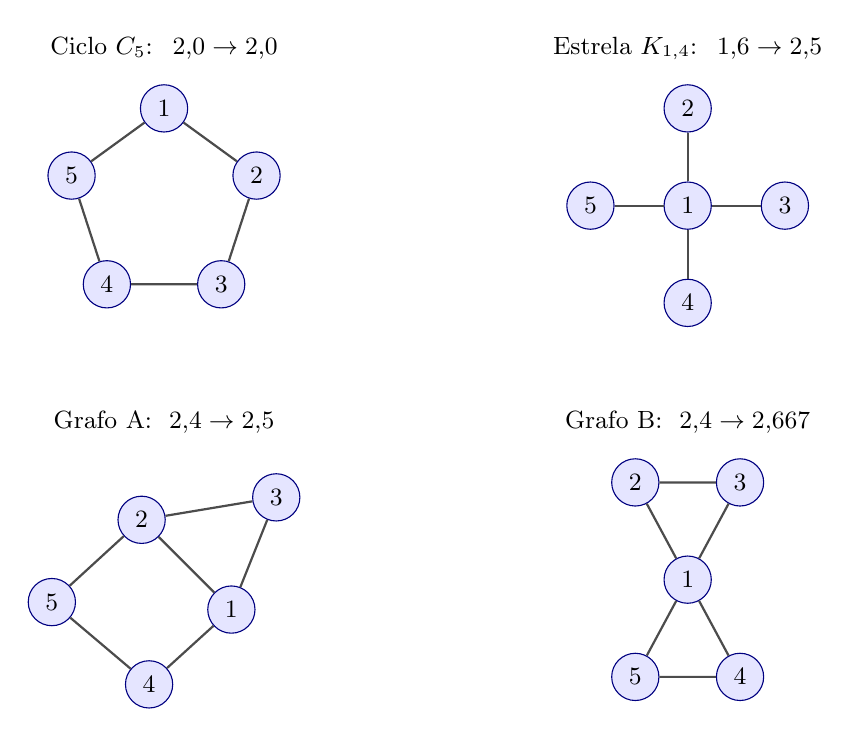
\begin{tikzpicture}[scale=0.95]
  % Ciclo C5
  \begin{scope}[shift={(0,0)}]
    \node at (0,2.1) {\small Ciclo $C_5$: \ $2{,}0 \to 2{,}0$};
    \foreach \i in {1,...,5} \node[v] (c\i) at ({90-72*(\i-1)}:1.3) {\i};
    \draw[e] (c1)--(c2)--(c3)--(c4)--(c5)--(c1);
  \end{scope}
  % Estrela K14
  \begin{scope}[shift={(7,0)}]
    \node at (0,2.1) {\small Estrela $K_{1,4}$: \ $1{,}6 \to 2{,}5$};
    \node[v] (s1) at (0,0) {1};
    \node[v] (s2) at (0,1.3) {2};
    \node[v] (s3) at (1.3,0) {3};
    \node[v] (s4) at (0,-1.3) {4};
    \node[v] (s5) at (-1.3,0) {5};
    \foreach \j in {2,...,5} \draw[e] (s1)--(s\j);
  \end{scope}
  % Grafo A
  \begin{scope}[shift={(0,-5)}]
    \node at (0,2.1) {\small Grafo A: \ $2{,}4 \to 2{,}5$};
    \node[v] (a1) at (0.9,-0.4) {1};
    \node[v] (a2) at (-0.3,0.8) {2};
    \node[v] (a3) at (1.5,1.1) {3};
    \node[v] (a4) at (-0.2,-1.4) {4};
    \node[v] (a5) at (-1.5,-0.3) {5};
    \draw[e] (a1)--(a2) (a1)--(a3) (a1)--(a4) (a2)--(a3) (a2)--(a5) (a4)--(a5);
  \end{scope}
  % Grafo B
  \begin{scope}[shift={(7,-5)}]
    \node at (0,2.1) {\small Grafo B: \ $2{,}4 \to 2{,}667$};
    \node[v] (b1) at (0,0) {1};
    \node[v] (b2) at (-0.7,1.3) {2};
    \node[v] (b3) at (0.7,1.3) {3};
    \node[v] (b4) at (0.7,-1.3) {4};
    \node[v] (b5) at (-0.7,-1.3) {5};
    \draw[e] (b1)--(b2) (b1)--(b3) (b1)--(b4) (b1)--(b5) (b2)--(b3) (b4)--(b5);
  \end{scope}
\end{tikzpicture}
\caption{Os quatro grafos de exemplo. Acima de cada desenho, o primeiro
número é a média por pessoa ($\dm$) e o segundo é a média dos graus
dos amigos ($\dA$).}\label{fig:exemplos}

{\footnotesize Fonte: elaboração própria.}
\end{figure}

\subsection{Toda lista de números é uma sequência de graus?}

Nos exemplos acima, sabemos que os grafos A e B existem porque
mostramos as arestas e o desenho. Mas, se alguém nos desse só uma lista
de números, como saber se existe um grafo simples com esses graus? Uma
lista com essa propriedade se chama \emph{sequência gráfica}.

Algumas condições são óbvias: pelo aperto de mãos, a soma tem que ser
par; e nenhum grau pode passar de $n-1$, já que ninguém tem mais amigos
do que o número de outras pessoas. Mas essas condições não bastam. A
lista $(3,3,1,1)$ tem soma par e nenhum grau maior que 3, porém não é
gráfica: os dois vértices de grau 3 teriam que ser ligados a todos os
outros, e então os dois últimos vértices teriam grau 2, e não 1.

Existe um procedimento simples para decidir isso, conhecido como
\emph{algoritmo de Havel-Hakimi} \cite{havel,hakimi}:
\begin{enumerate}
  \item ordene a lista do maior para o menor;
  \item tire o primeiro número, digamos $r$, e subtraia 1 dos $r$ números seguintes
        (isso corresponde a ligar o vértice de maior grau aos $r$ vértices de maior grau restantes);
  \item repita com a lista nova.
\end{enumerate}
Se em algum momento aparecer um número negativo, ou não houver números
suficientes para subtrair, a lista não é gráfica. Se a lista virar só
zeros, ela é gráfica.

Para o grafo A: $(3,3,2,2,2) \to (2,1,1,2)$, que reordenada fica
$(2,2,1,1) \to (1,0,1)$, que reordenada fica $(1,1,0) \to (0,0)$.
Terminou em zeros, então é gráfica. Para B:
$(4,2,2,2,2)\to(1,1,1,1)\to(0,1,1)$, reordenando $(1,1,0)\to(0,0)$,
também gráfica. Já para $(3,3,1,1)$: tirando o 3, ficamos com
$(2,0,0)$; tirando o 2, teríamos que subtrair 1 de dois zeros, o que dá
números negativos. Então $(3,3,1,1)$ não é gráfica, como já tínhamos
visto.

% ------------------------------------------------------------
\section{Simulação no computador}\label{sec:simulacao}
% ------------------------------------------------------------

Para ver o paradoxo em redes maiores, escrevemos um programa em Python
usando a biblioteca NetworkX \cite{networkx}. O código está no arquivo
\texttt{simulacao\_paradoxo\_amizade.py}, entregue junto com este trabalho.

\subsection{Três redes de 300 pessoas}

Geramos três redes artificiais com 300 pessoas cada,
utilizando o algoritmo de Havel-Hakimi para construir
grafos a partir de sequências de graus. As sequências
foram elaboradas para representar três padrões diferentes
de distribuição de amizades:

\begin{itemize}
    \item \textbf{Anel com atalhos:} sequência inspirada
    em uma rede circular na qual cada pessoa possui
    inicialmente seis amigos, com alterações aleatórias
    que produzem pequenas variações nos graus.

    \item \textbf{Sorteio de pares:} sequência de graus
    gerada a partir de sorteios independentes, buscando
    aproximar uma distribuição binomial.

    \item \textbf{Rede com populares:} sequência produzida
    por um processo de crescimento em que novas pessoas
    estabelecem três amizades, dando preferência a pessoas
    com graus maiores.
\end{itemize}

Esses padrões são inspirados, respectivamente, nos modelos
de Watts-Strogatz \cite{ws}, Erdős-Rényi \cite{er} e
Barabási-Albert \cite{ba}. Entretanto, as conexões finais
são determinadas pelo algoritmo de Havel-Hakimi, de modo
que os grafos construídos não correspondem necessariamente
às estruturas originais desses modelos.

Após a construção, analisamos os graus, suas médias e
variâncias, as médias por indicação e a conectividade
dos grafos.


\begin{table}[htbp]
\centering
\caption{Médias e propriedades das três redes geradas
com Havel--Hakimi ($n=300$).}
\label{tab:redes}
\begin{tabular}{lcccccccc}
\toprule
Rede & $m$ & $\bar d$ & $\sigma^2$ & $\bar d_A$
& $\bar d_I$ & Isol. & Comp. & Maior \\
\midrule
Anel com atalhos
& 900 & 6,000 & 0,567 & 6,094 & 6,009
& 0 & 1 & 300 \\
Sorteio de pares
& 938 & 6,253 & 5,656 & 7,158 & 6,305
& 1 & 11 & 266 \\
Com populares
& 891 & 5,940 & 32,783 & 11,459 & 7,088
& 0 & 33 & 172 \\
\bottomrule
\end{tabular}

\smallskip
{\footnotesize
Isol.: vértices isolados;
Comp.: componentes conexas;
Maior: número de vértices na maior componente.
Fonte: elaboração própria.}
\end{table}

\begin{figure}[htbp]
    \centering

    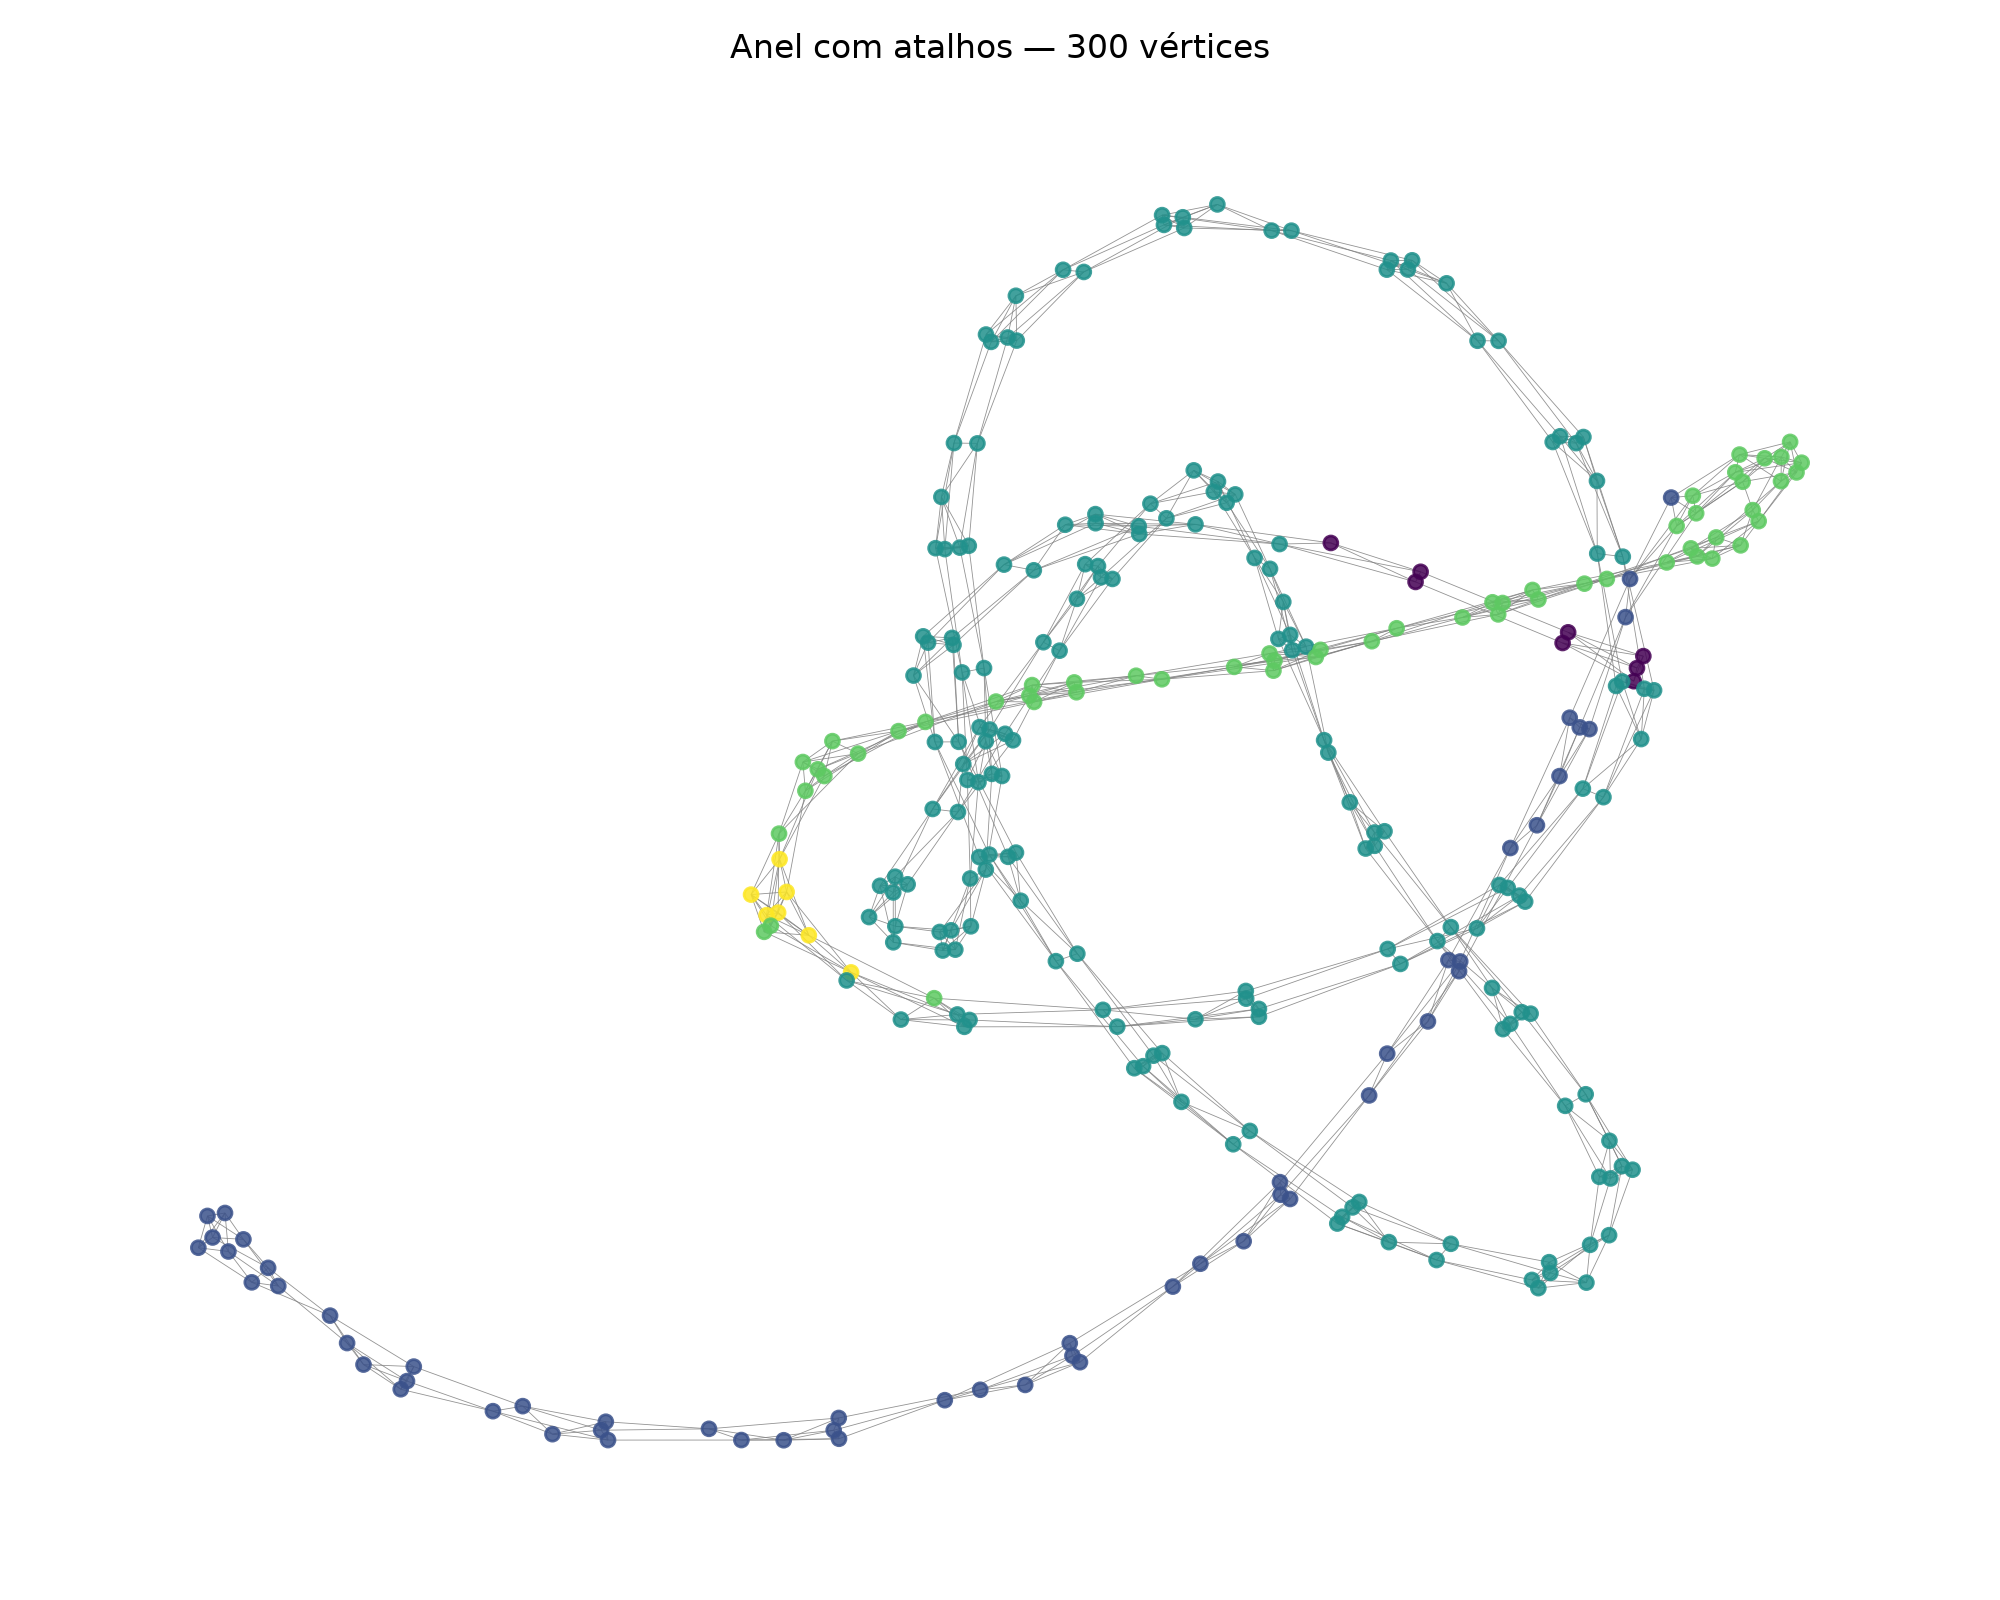
\includegraphics[width=0.3\textwidth]{grafo_anel.png}
    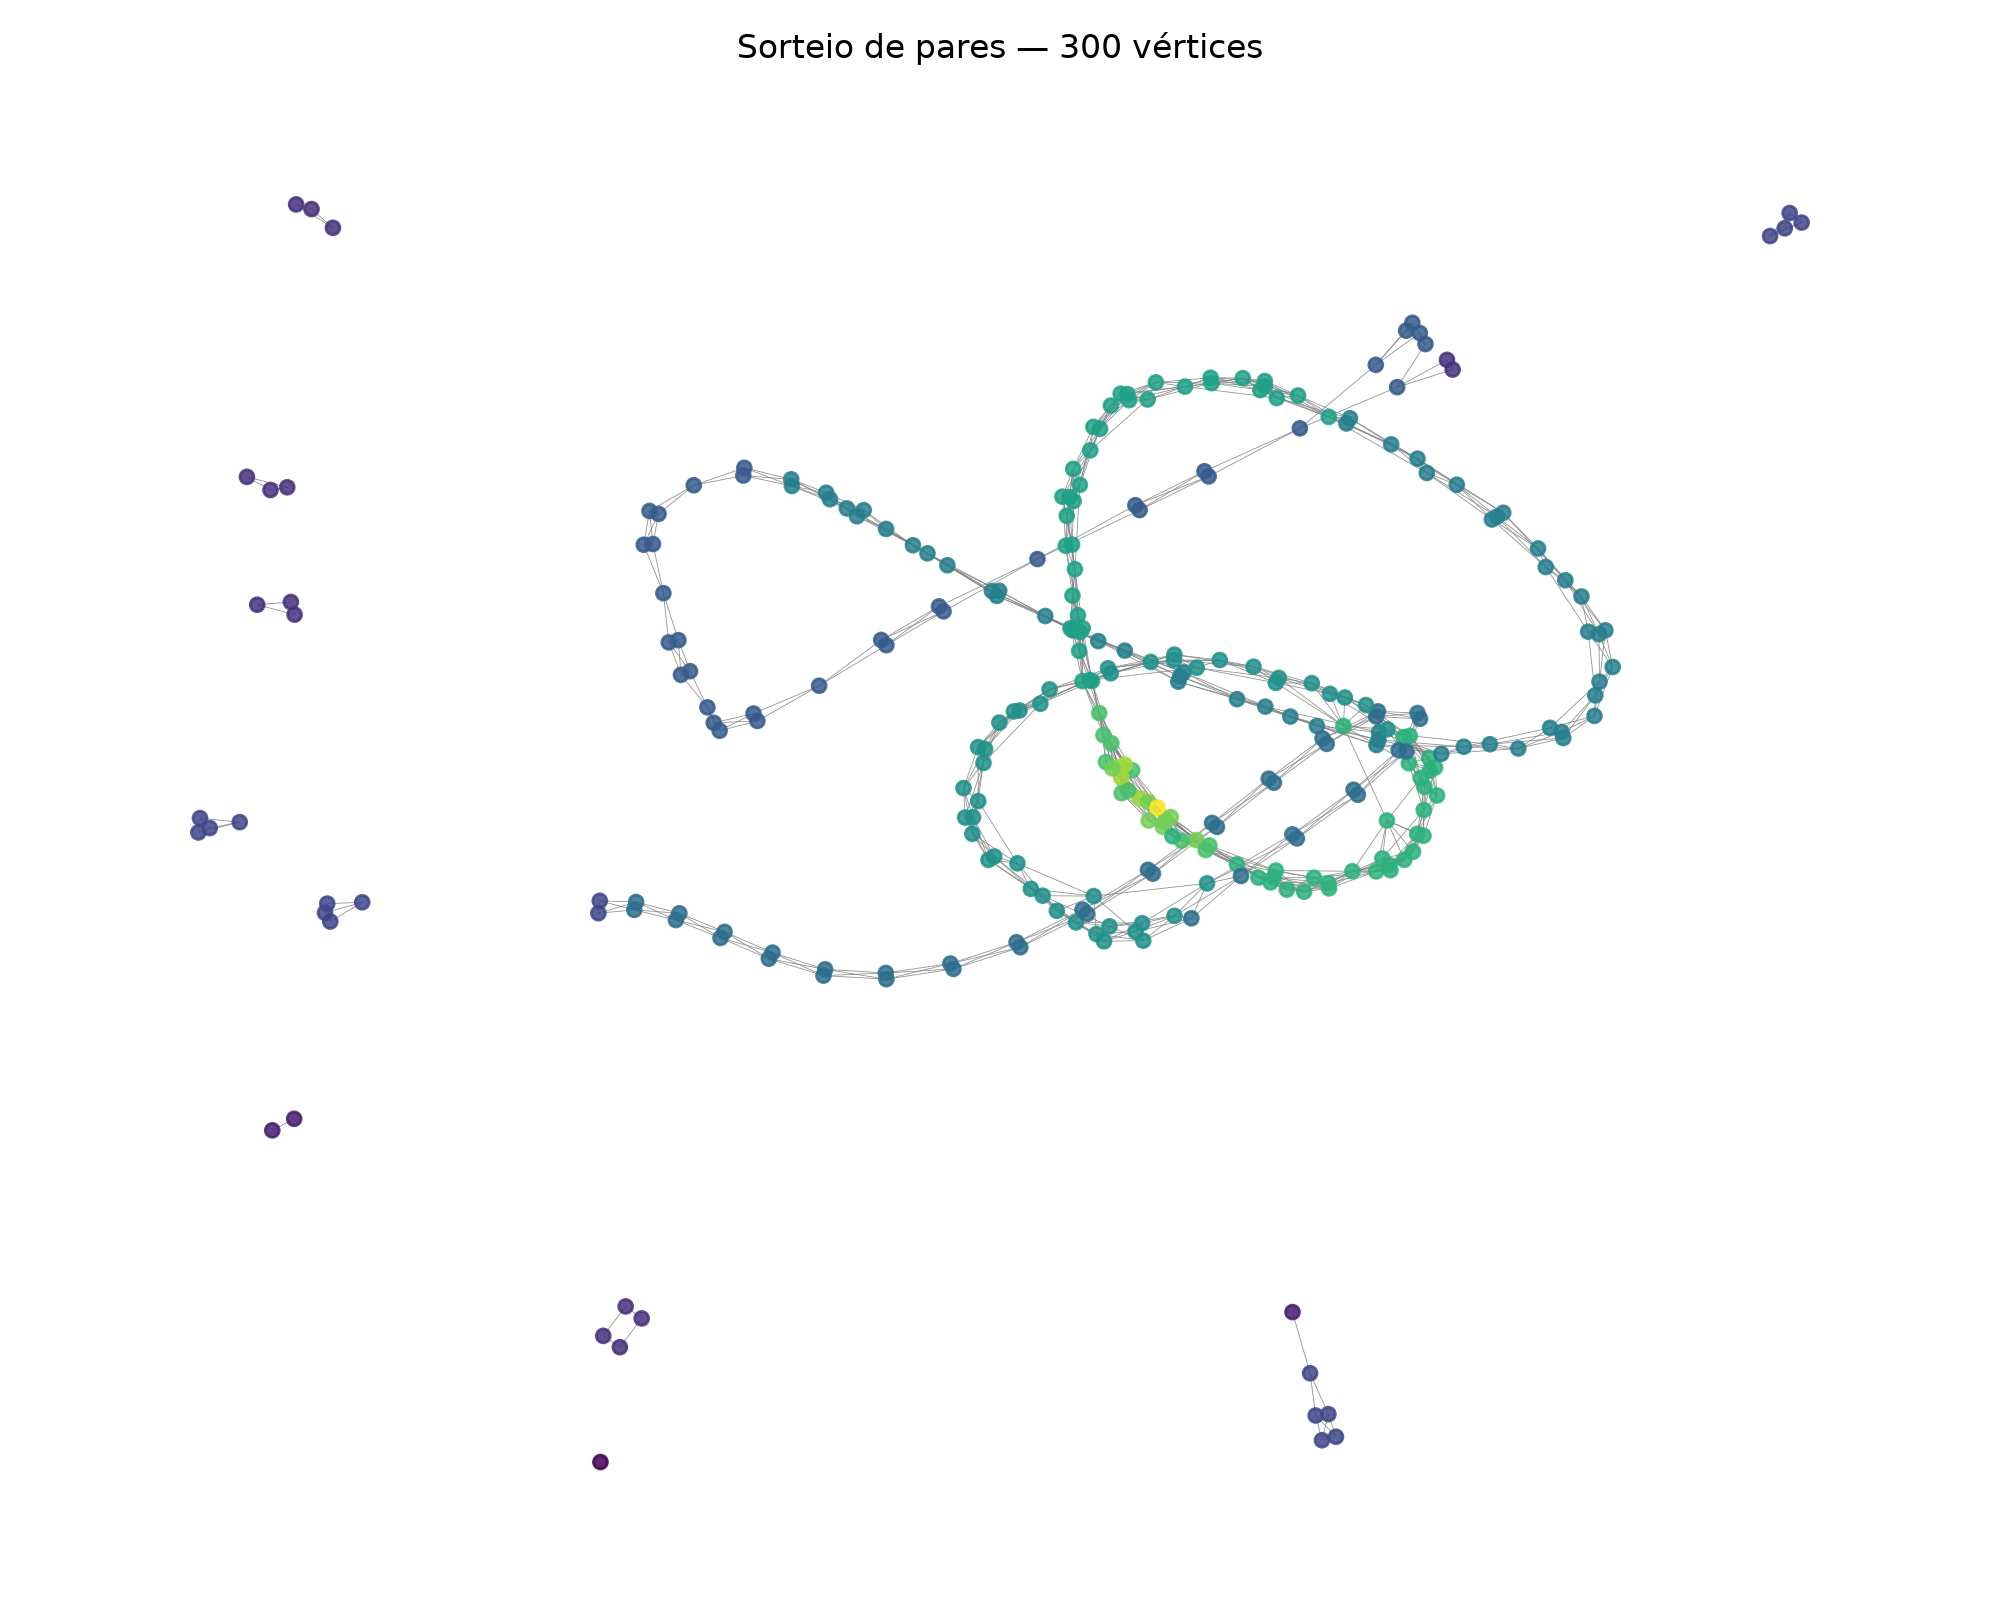
\includegraphics[width=0.3\textwidth]{grafo_pares.png}
    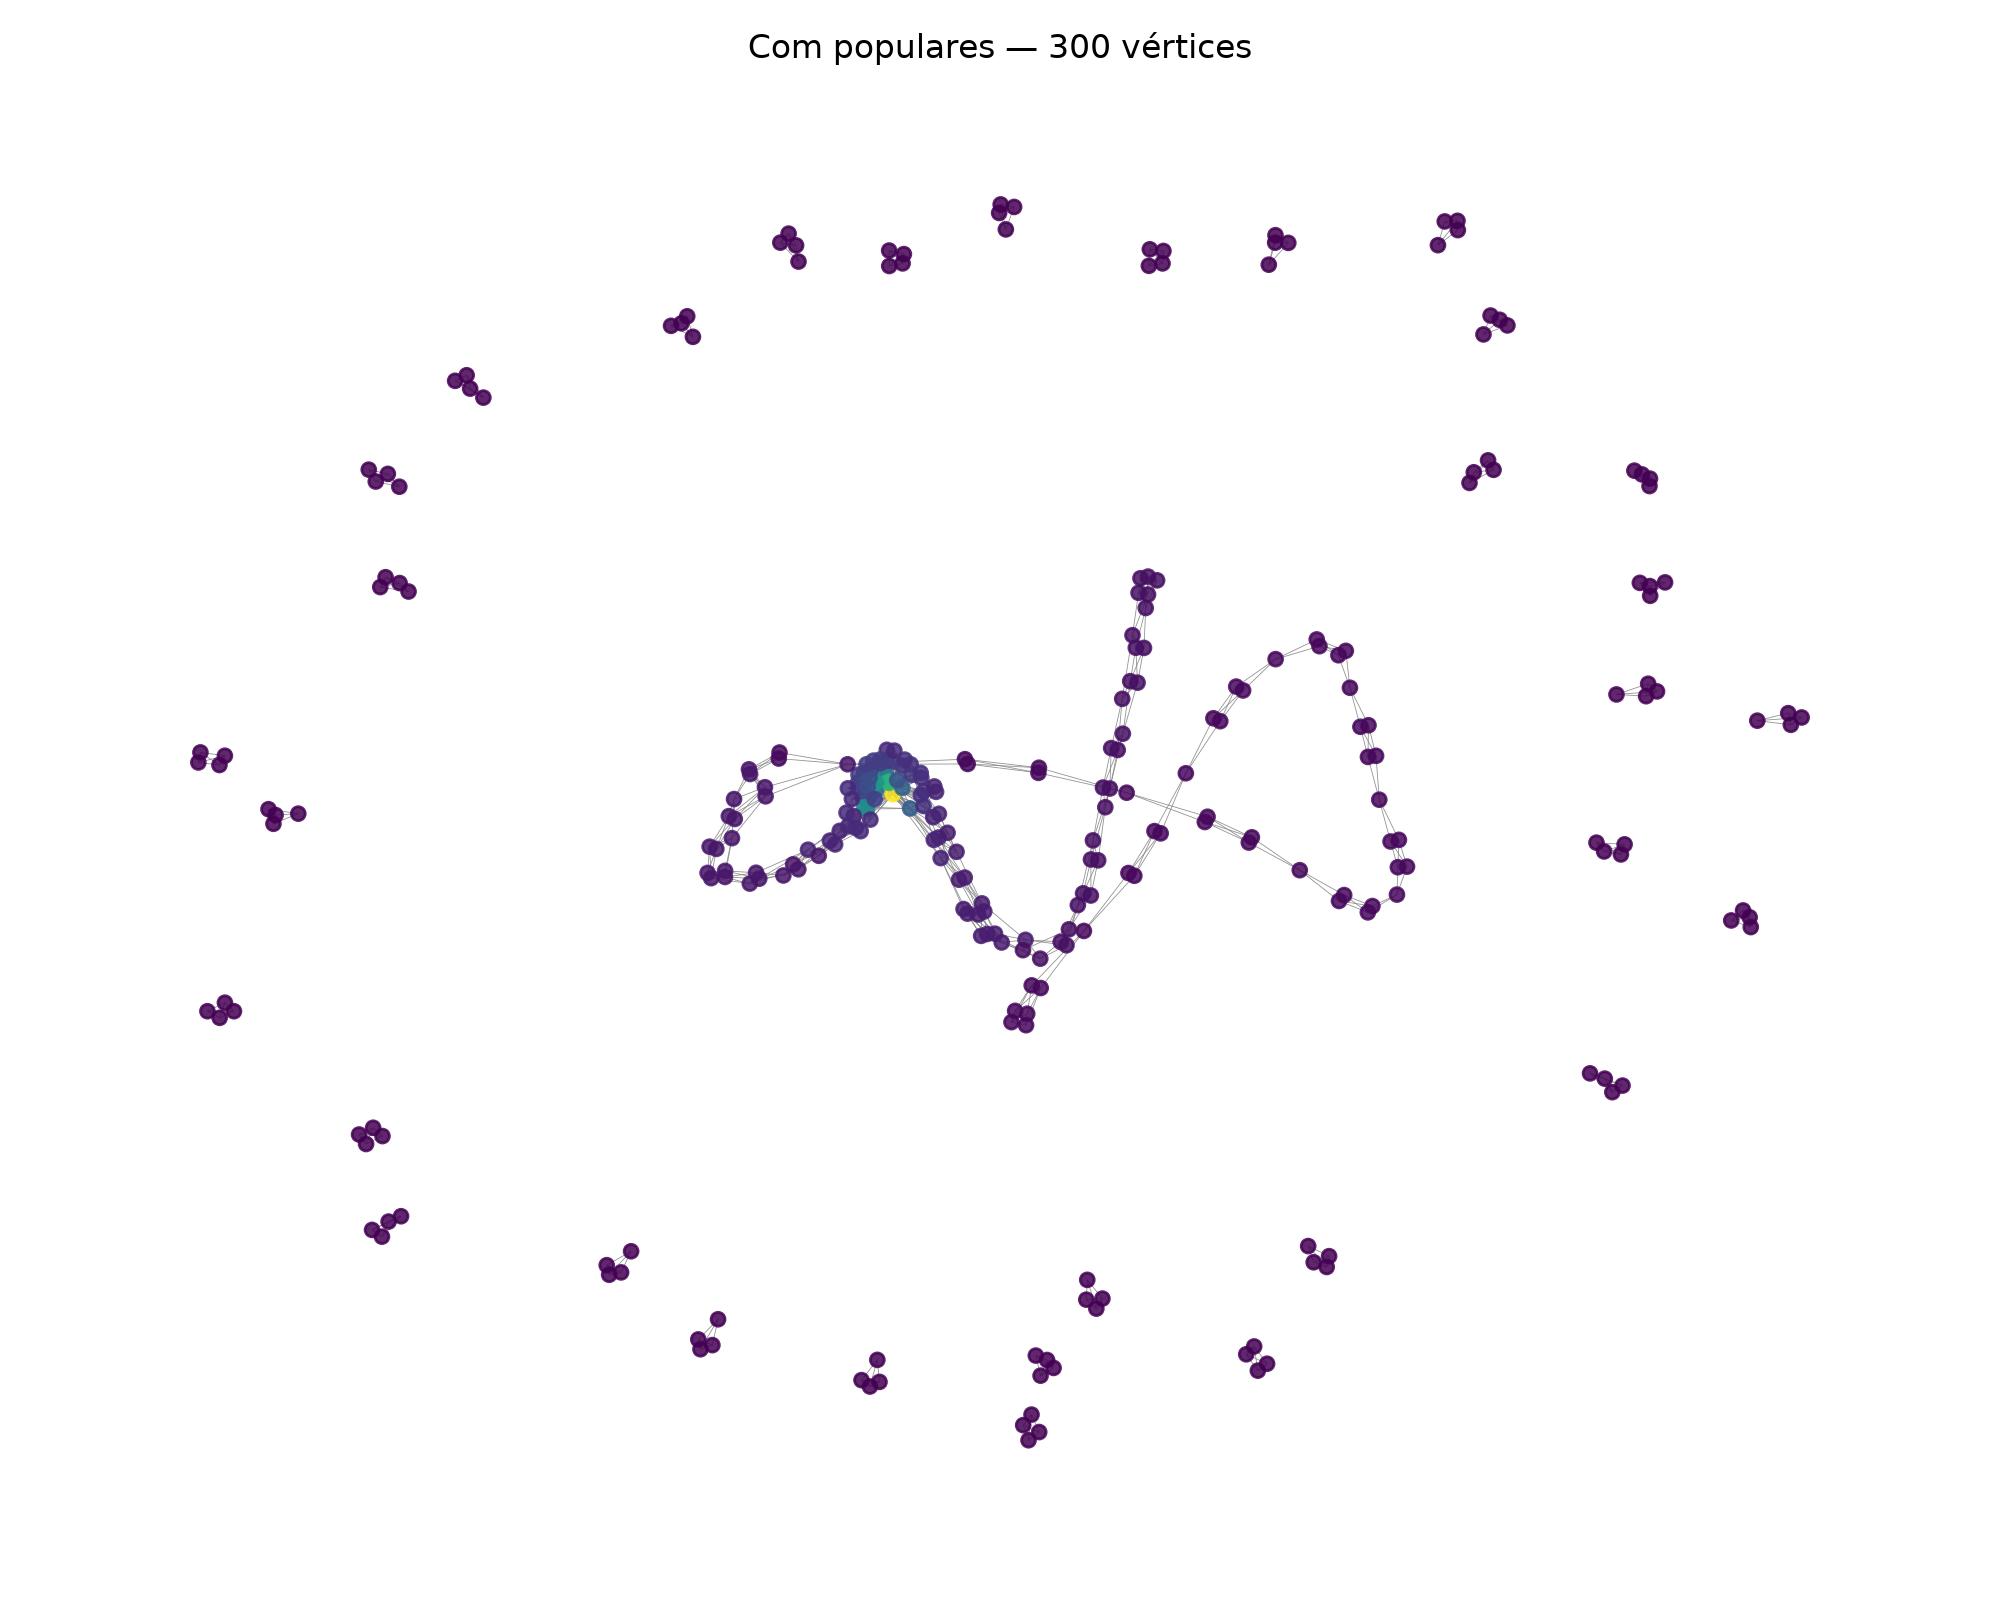
\includegraphics[width=0.3\textwidth]{grafo_populares.png}

    \caption{Representações das três redes de 300 vértices
    construídas pelo algoritmo de Havel-Hakimi.
    As cores dos vértices representam seus graus, e
    a posição dos vértices foi determinada pelo
    algoritmo de visualização spring layout.}

    \label{fig:redes}

    \smallskip
    {\footnotesize Fonte: elaboração própria.}
\end{figure}
As três redes apresentam médias de graus próximas de 6,
mas possuem variâncias bastante diferentes. No anel com
atalhos, a variância é pequena ($\sigma^2=0{,}567$), e a
média dos graus dos amigos ($\dA=6{,}094$) fica próxima
da média geral. Na rede com populares, a variância é muito
maior ($\sigma^2=32{,}783$), fazendo com que a média dos
graus dos amigos ($\dA=11{,}459$) seja quase o dobro da
média dos graus das pessoas ($\dm=5{,}940$).

Esses resultados confirmam a relação demonstrada pelo
Teorema~\ref{teo:principal}, segundo a qual a diferença
entre as médias depende da variância dos graus dividida
pela média dos graus.

Além disso, verificamos diferenças na conectividade.
O anel com atalhos possui apenas uma componente conexa,
enquanto a rede de sorteio de pares possui 11 e a rede
com populares possui 33. Isso mostra que a distribuição
dos graus não determina, sozinha, a conectividade da rede.

Na rede de sorteio de pares, encontramos um vértice
isolado. Por isso, a média por indicação foi calculada
considerando apenas os 299 vértices com pelo menos um
amigo, conforme discutido anteriormente.


\subsection{Aplicação: espalhar uma notícia}

Uma consequência prática do paradoxo é a seguinte: se queremos espalhar
uma informação numa rede e só podemos avisar poucas pessoas no início,
pode valer a pena escolher essas pessoas \emph{por indicação} em vez de
sorteá-las diretamente, porque quem é indicado tende a ter mais amigos.

Testamos isso nas três redes. Escolhemos 15 pessoas para receber a
notícia no início, de dois jeitos:
\begin{itemize}
  \item \textbf{Direto:} sorteamos 15 pessoas diferentes ao acaso.
  \item \textbf{Por indicação:} sorteamos uma pessoa e ela indica um
        amigo ao acaso; repetimos até ter 15 pessoas indicadas
        diferentes.
\end{itemize}
Depois, a notícia se espalha em 4 rodadas. Em cada rodada, quem acabou
de saber a notícia tenta contá-la a cada amigo que ainda não sabe, e
consegue com probabilidade $0{,}15$. Ao final, contamos quantas pessoas
souberam (incluindo as 15 iniciais). Repetimos tudo 500 vezes para cada
rede e cada jeito de escolher, e calculamos as médias
(Tabela~\ref{tab:noticia}).


\begin{table}[htbp]
\centering
\caption{Grau médio das 15 pessoas iniciais e
porcentagem média da rede informada após
4 rodadas (500 repetições).}
\label{tab:noticia}
\begin{tabular}{lcccc}
\toprule
& \multicolumn{2}{c}{Grau médio inicial}
& \multicolumn{2}{c}{Alcance (\%)} \\
\cmidrule(lr){2-3}
\cmidrule(lr){4-5}
Rede & Direto & Indicação & Direto & Indicação \\
\midrule
Anel com atalhos
& 6,00 & 6,01 & 14,15 & 14,20 \\
Sorteio de pares
& 6,30 & 6,30 & 16,26 & 16,12 \\
Com populares
& 5,94 & 6,96 & 20,11 & 20,54 \\
\bottomrule
\end{tabular}

\smallskip
{\footnotesize Fonte: elaboração própria.}
\end{table}


Na rede com populares, as pessoas selecionadas por
indicação apresentaram grau médio de 6,96, contra 5,94
no sorteio direto. O alcance médio da notícia também
foi maior, passando de 20,11\% para 20,54\%.

Nas outras duas redes, os resultados foram bastante
próximos. No anel com atalhos, o alcance passou de
14,15\% para 14,20\%. Já na rede de sorteio de pares,
a indicação apresentou alcance ligeiramente inferior
ao sorteio direto, com 16,12\% contra 16,26\%.

Esses resultados mostram que, embora o Paradoxo da
Amizade favoreça a seleção de pessoas com mais conexões,
isso não garante uma propagação significativamente
maior da informação.

O alcance depende também da organização das amizades
e da conectividade do grafo. Na rede com populares,
por exemplo, foram encontradas 33 componentes conexas,
o que limita a propagação entre diferentes grupos.

Portanto, a simulação ilustra uma possível aplicação
do paradoxo, mas também evidencia que a quantidade
de conexões não é o único fator responsável pela
eficiência da divulgação de informações.

% ------------------------------------------------------------
\section{Conclusão}

A sensação de que ``meus amigos têm mais amigos do que eu''
tem uma explicação matemática: quando olhamos a rede
através das amizades, cada pessoa é contada uma vez
para cada amigo que tem, e as pessoas populares
pesam mais. Provamos que a média dos graus dos amigos é

\[
\dA = \dm + \frac{\sigma^2}{\dm},
\]

e portanto nunca é menor que a média dos graus das
pessoas, sendo igual apenas quando todos têm o mesmo
número de amigos. Provamos também um resultado semelhante
quando sorteamos uma pessoa e pedimos que ela indique
um amigo.

Os exemplos pequenos e as simulações confirmam que
o Paradoxo da Amizade se torna mais evidente quando
existe maior desigualdade entre os graus dos vértices.
A aplicação do algoritmo de Havel-Hakimi permitiu
construir redes artificiais a partir de diferentes
sequências de graus e analisar como a distribuição
das amizades se relaciona com esse fenômeno.

Na simulação de propagação de uma notícia, observamos
que a seleção por indicação pode favorecer a escolha
de pessoas com mais conexões. Entretanto, essa vantagem
não resultou necessariamente em um aumento expressivo
do alcance da informação, mostrando que a conectividade
e a estrutura das redes também influenciam o processo.

Dessa forma, o trabalho demonstra matematicamente o
Paradoxo da Amizade e apresenta uma aplicação computacional
envolvendo sequências gráficas, o algoritmo de
Havel-Hakimi, componentes conexas e propagação de
informações em grafos.
% -----------------------------------------------------------
\newpage
\phantomsection
\addcontentsline{toc}{section}{Referências}
\begin{thebibliography}{9}
\singlespacing

\bibitem{feld}
FELD, Scott L. Why your friends have more friends than you do.
\emph{American Journal of Sociology}, v.~96, n.~6, p.~1464--1477, 1991.

\bibitem{havel}
HAVEL, Václav. A remark on the existence of finite graphs.
\emph{Časopis pro pěstování matematiky}, v.~80, n.~4, p.~477--480, 1955.

\bibitem{hakimi}
HAKIMI, S.~L. On the realizability of a set of integers as degrees of
the vertices of a linear graph. I. \emph{Journal of the Society for
Industrial and Applied Mathematics}, v.~10, n.~3, p.~496--506, 1962.

\bibitem{networkx}
HAGBERG, Aric A.; SCHULT, Daniel A.; SWART, Pieter J. Exploring network
structure, dynamics, and function using NetworkX. In: \emph{Proceedings
of the 7th Python in Science Conference (SciPy 2008)}. Pasadena, 2008.
p.~11--15.


\bibitem{ws}
WATTS, Duncan J.; STROGATZ, Steven H. Collective dynamics of
`small-world' networks. \emph{Nature}, v.~393, p.~440--442, 1998.

\bibitem{er}
ERDŐS, Paul; RÉNYI, Alfréd. On random graphs I. \emph{Publicationes
Mathematicae Debrecen}, v.~6, p.~290--297, 1959.

\bibitem{ba}
BARABÁSI, Albert-László; ALBERT, Réka. Emergence of scaling in random
networks. \emph{Science}, v.~286, p.~509--512, 1999.

\end{thebibliography}

\end{document}
